\chapter{The World Needs Changes or Application Customisation}\label{ch00:03}

\myepigraph{Technical skill is mastery of complexity, while creativity is mastery of simplicity.}{Erik Christopher Zeeman}

  Before making any changes to the generated applications, we should discussed its modules, which are typical for any TG-based application project, their roles and interdependencies.

\section{Project Modules}
  The generated application consists of six modules with interdependencies depicted in Fig.~\ref{img:ch00:03:project_module_dependencies}.
  These modules are grouped into three independent groups: Server Modules, Client Modules and Shared Module.
  
  \begin{description}
    \item[\textbf{Shared Module.}] Includes a single module \texttt{coolapp-pojo-bl}, which is independent from other application modules, and is shared between the other two groups.
	This module represents the very core of the application where the business domain model is defined.   
    \item[\textbf{Server Modules.}] Include two modules -- \texttt{coolapp-dao} and \texttt{coolapp-web-server} -- that together define the application web server.	
      \begin{itemize}
	\item \texttt{coolapp-dao} -- contains Data Access Objects (DAO), which are the database-aware implementations of controllers defined as part of the \texttt{coolapp-pojo-bl} module; designed to support domain driven unit testing, which makes it a natural choice for data-oriented unit tests.
	\item \texttt{coolapp-web-server} -- represents an entry point for the server-side application; has a transitive dependency to module \texttt{coolapp-pojo-bl} via a direct dependency to \texttt{coolapp-dao}; registers web resources associated with domain entities, which bind together controllers with their DAO implementations.
      \end{itemize}
    \item[\textbf{Client Modules.}] Include three modules~--~\texttt{coolapp-rao}, \texttt{coolapp-ui} and \texttt{coolapp-web-client}~--~that together define the application web client.
      \begin{itemize}
	\item \texttt{coolapp-rao} -- contains (web) Resource Access Objects (RAO), which are HTTP-aware implementations of controllers defined as part of the \texttt{coolapp-pojo-bl} module, which is its only dependency.
	\item \texttt{coolapp-ui} -- contains User Interface elements such as frames, panels, menu items.
	\item \texttt{coolapp-web-client} -- represents an entry point for the client-side application; has a transitive dependency to module \texttt{coolapp-pojo-bl} via a direct dependency to \texttt{coolapp-rao} and \texttt{coolapp-ui}; binds together controllers defined in \texttt{coolapp-pojo-bl} with their RAO implementation, which ensures resolution of contract dependencies in \texttt{coolapp-ui}.
      \end{itemize}
   \end{description}

\begin{image}{Dependencies between Project Modules.}{\label{img:ch00:03:project_module_dependencies}}    
    \scalebox{1.0} {
  \begin{tikzpicture}
    \draw[very thick, dashed, color=blue!50!black, rounded corners] (-2.3, 1.8) rectangle (10.7,-1.2);
    \node[rotate=90,color=blue!50!black] at (-2.6, 0.25) {\small Server Modules};

    \umlbasiccomponent[x=0, y=0, fill=blue!10]{coolapp-dao}
    \umlbasiccomponent[x=8, y=0, fill=blue!10]{coolapp-web-server}

    \draw[very thick, dashed, color=red!50!black, rounded corners] (1.8, -3.3) rectangle (6.2,-6.1);
    \node[color=red!50!black] at (4.9, -3) {\small Shared Module};
    \umlbasiccomponent[x=4, y=-5]{coolapp-pojo-bl}
    
    \umlnote[x=-2, y=3.5, width=5.5cm, fill=annotationbgcolor]{coolapp-dao}{\scriptsize Date Access Objects layer, which provides RDBMS-based implementation for domain controllers.}
    \umlnote[x=-2, y=-3.5, width=5.5cm, fill=annotationbgcolor]{coolapp-pojo-bl}{\scriptsize Defines business domain model (entities and controllers), shared between client and server tiers.}

    \umluniassoc{coolapp-dao}{coolapp-pojo-bl}
    \umluniassoc[name=w2d]{coolapp-web-server}{coolapp-dao}
    \umlnote[x=5, y=3.5, width=5.5cm, fill=annotationbgcolor]{w2d-1}{\scriptsize Web resources use DB driven implementation of domain controllers} 

    \draw[very thick, dashed, color=green!50!black, rounded corners] (-1, -8.1) rectangle (8.9,-15.2);
    \node[rotate=90,color=green!50!black] at (-1.3, -9.7) {\small Client Modules};

    \umlbasiccomponent[x=7, y=-10, fill=green!30]{coolapp-ui}
    \umlbasiccomponent[x=1, y=-10, fill=green!30]{coolapp-rao}
    \umlbasiccomponent[x=4, y=-14, fill=green!30]{coolapp-web-client}   

    \umlnote[x=-2, y=-6.5, width=5.5cm, fill=annotationbgcolor]{coolapp-rao}{\scriptsize Resource Access Objects, which provides HTTP-based implementation for domain controllers.}
    \umlnote[x=-3, y=-13.7, width=3cm, fill=annotationbgcolor]{coolapp-web-client}{\scriptsize Binds together UI and RAO implementation of domain controllers to define a web client application.}

    \umluniassoc[name=u2m]{coolapp-ui}{coolapp-pojo-bl}
    \umlnote[x=9, y=-6, width=3.5cm, fill=annotationbgcolor]{u2m-1}{\scriptsize Accessed domain model and controller via their contracts (not implementation).} 
    \umluniassoc{coolapp-rao}{coolapp-pojo-bl}
    \umluniassoc{coolapp-web-client}{coolapp-ui}
    \umluniassoc{coolapp-web-client}{coolapp-rao}  

  \end{tikzpicture}
  }
  \end{image}

  The role for each module is well defined and serves as one of the aspects of the TG development model.
  The core value of the application is in its business domain model.
  Module \texttt{coolapp-pojo-bl} is used for defining all domain entity types, validation and controller contracts that model the business domain for which the application is being constructed.
  Each domain entity type is associated with a corresponding CRUD (Create Request Update Delete) controller contract, which serves as the primary way to interact with domain entities.
  The \texttt{coolapp-rao} and \texttt{coolapp-dao} module fulfil client and server side implementation of domain controllers respectively.
  All essential functionality for CRUD controllers is provided by the platform, and is reused by sub-typing corresponding platform classes.\footnote{Later chapters provide all details on how this is done, how to properly reuse and customise provided functionality.}.
  There are guidelines as to what logic is better suited for the client side and what for the server side of the applicaton.
  These are provided in later chapters of this book.  

\section{Quick changes}

  In order to provide a sense of what it is like to change TG-based application let's consider one of the entity types, which is provided as part of the generated application -- \emph{Person} -- listed in Listing~\ref{lst:Person}.

 \lstset{language=Java,
	  escapechar=\%,
	  numbers=left, numberstyle=\tiny, basicstyle=\scriptsize\color{basiccolor}, stepnumber=1, numbersep=5pt, keywordstyle=\bfseries\color{codefgcolor}, stringstyle=\color{stringcolor}}
  \begin{code}{A fragment of entity type Person.}{\label{lst:Person}}{codebgcolor}
    \begin{lstlisting}
@KeyType(String.class)
@KeyTitle(value = "Person Code", desc = "A code uniquely representing a person.")
@DescTitle(value = "Description", desc = "A short description...")
@MapEntityTo("CRAFT")
@DefaultController(IPerson.class)
public class Person extends AbstractEntity<String> {
    .....................
    @IsProperty
    @Title(value = "Username", desc = "Application user name")
    @MapTo("USER_NAME")
    private String username;
    .....................
}
    \end{lstlisting}
  \end{code}
  
  The purpose of entity Person is to model a concept of a person that is either using the application or needs referenced by any other domain entity, which might be required by some business process implemented in the application.
  The platform provides a concept of the application user, which is implemented by entity \emph{User}.
  This entity is an integral part of the platform and cannot be changed in any derived application\footnote{More detailed on entity User is provided as part of security related chapter.}.
  The Person entity reuses this User concept by sharing some of its properties.
  Specifically, property \emph{username} and \emph{password}.
  This way Person and User fuse together, which is not required, but convenient.  

\subsection{Attributes for Entity and its Properties}
  Any custom Java type that subtypes \emph{AbstractEntity} is an entity from platform perspective.
  Type AbstractEntity is very rich in its functionality and provides full support for modeling a wide variety of business domain entities.
  It is discussed in great details further in the book.
  So, here we just touch on some of the aspects of domain entity modeling.

  Domain entities may have \emph{simple} or \emph{composite} (more than property is involved) business key, which uniquely identifies each entity instance.
  Entity Person has a simple business key of type String, which is specified by annotation \emph{KeyType}  and \emph{AbstractEnity} type parameter as can be observed in Listing~\ref{lst:Person} at lines 1 and 6.
  
  Each property of domain entities can be provided with a user friendly title and description, which is used by the system when building UI or reporting warnings/errors.
  This is done by annotating property representing fields with annotation \emph{Title} such as depicted in Listing~\ref{lst:Person} at line 9.
  However, property \emph{key}, which implements the business key concept, is declared at the AbstractEntity level, and thus not accessible for modification from custom types such as Person.
  Another inherited property is \emph{desc}, which represents a description for an entity instance.
  
  In order to provide uniform customisation capabilities for all entity properties, special entity type annotations \emph{KeyTitle} and \emph{DescTitle} are provided and should be used in a way depicted in Listing~\ref{lst:Person} at lines 2 and 3.
  
  \paragraph*{Property title change.}
  Let's change the description of property \emph{username} from \texttt{Username} to \texttt{Login Name}, and description from \texttt{Application user name} to \texttt{A name, which is used for loging into the application}.
  In order to do this, locate type Person by pressing the key combination \texttt{Ctrl+Shift+T} to invoke \emph{Open Type} dialog and type \emph{Person} (refer Fig.~\ref{img:ch00:03:open-type-dialog}), which should quickly locate the required type.

  \begin{image}{Open Type Dialog.}{\label{img:ch00:03:open-type-dialog}}
    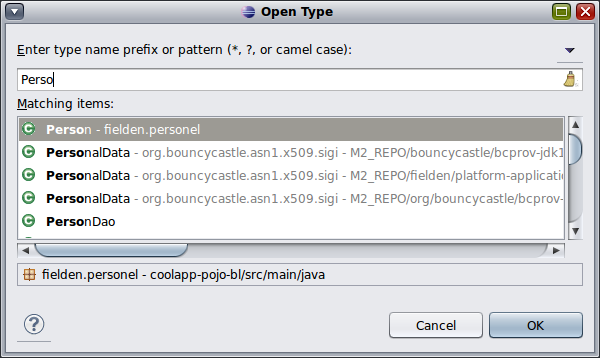
\includegraphics[width=0.6\textwidth]{parts/00-part/chapters/02-making-changes/images/01-open-type-person.png}
  \end{image}

  Open the type, make the changes in the code editor and save your them.
  In order to see the effect run the application from Eclipse IDE.
  This requires starting both the server (if it is not already running) and the client applications.
  The client application needs to be restarted is it was running at the time of changes in order to reload the recompiled classes.
  Although, the modified classes are shared between client and server applications, their reloading by the server is not essential as the performed changes effect only the client side.
  
  Once the client is up and running, go to \emph{Table Codes}$\longrightarrow$\emph{Personnel} and observer the affect of your changes, which should be obvious in the grid, selection criteria panel and in the configuration domain tree (can be invoked by clicking the \emph{Configure} button on Personnel Centre).
  
\subsection{Enhance Person and Test Your Changes}\label{ch00:03:the-scenario}
  Let's now make some more serious changes. 
  
  \subsubsection*{The scenario.}
  The following items should serve as a mini specification of the business rules for personnel enhancement.
  
  \begin{enumerate}
    \item Entity \emph{Person} should be provided with a non-mandatory property \emph{birthday}.
    \item This new property should be validated upon entry or change: 
	\begin{enumerate}
	  \item if the birth date value indicates that a person is too young (younger than 23 years of age) then a warning should be produced, but the value should be accepted;
	  \item no future birth dates should be accept.
	\end{enumerate}
  \end{enumerate}

  \subsubsection*{Implementing the requirements.}

  \paragraph*{Adding property.} 
  In order to take the advantage of Eclipse's source templates, the platform includes a set of templates for automate commonly encountered situations when describing domain entities.
  These templates can be downloaded from the platform's web site at \url{http://www.fielden.com.ua/trac/pnl-tg/wiki/EclipseCodeTemplates}.
  
  If the Eclipse IDE was property setup with TG templates, then creation of a new property is trivial.
  Type \texttt{tgp} and hit \texttt{Ctrl+Space} in the code editor of type Person under the last available property.
  This should result in the dialog depicted in Fig.~\ref{img:ch00:03:gen-prop-template}, which should be used to select option \texttt{tgprop} for property template generation.

  \begin{image}{TG Property Templates Dialog.}{\label{img:ch00:03:gen-prop-template}}
    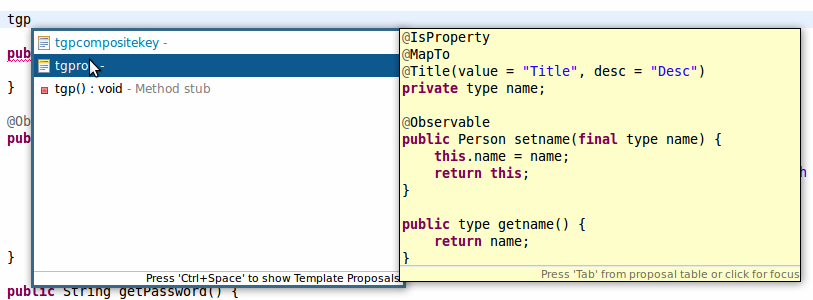
\includegraphics[width=0.8\textwidth]{parts/00-part/chapters/02-making-changes/images/02-birthday-property-gen.png}
  \end{image}

  The generation result is depicted in Fig.~\ref{img:ch00:03:prop-template}.
  Right after generation, the template is in edit mode, which means that all of its parts can be conveniently edited and navigated between using the \texttt{Tab} key.
  The first selected word is \emph{Title}, without moving the keyboard cursor or clicking anywhere with the mouse, start typing the new title \emph{Birthday}.
  Hit the \texttt{Tab} key to move to the \emph{desc} attribute and type \emph{The date when person was born}.
  Hit the \texttt{Tab} key again to move to the \emph{type} part and type \emph{Date} to specify the property type.
  Hit the \texttt{Tab} key to move to the \emph{name} and type \emph{birthday} to give the property a field name.
  The next \texttt{Tab} will move the cursor to the setter name between the word \emph{set} and \emph{birthday}.
  Hit \texttt{Enter} to confirm changes.
  At this stage both setter and getter have the \emph{birthday} portion starting with small \texttt{b}.
  Change it to be a capital \texttt{B}, so that the setter read \emph{setBirthday} and getter read \emph{getBirthday}.

  \begin{image}{TG Property Temple.}{\label{img:ch00:03:prop-template}}
    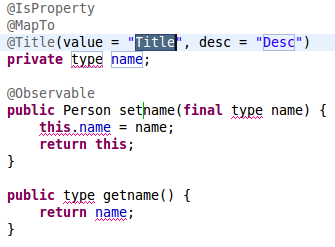
\includegraphics[width=0.4\textwidth]{parts/00-part/chapters/02-making-changes/images/03-birthday-property-template.png}
  \end{image}

  The final look of the property is provided in Listing~\ref{lst:Person-birthday}.
  Please note the return type of the setter, which matches the enclosing type Person.
  This is done to support method chaining, which is so convenient when creating new or modifying existing entity instances.

  \begin{code}{Property \emph{birthday}.}{\label{lst:Person-birthday}}{codebgcolor}
    \begin{lstlisting}
    @IsProperty
    @MapTo
    @Title(value = "Birthday", desc = "The date when person was born")
    private Date birthday;
    
    @Observable
    public Person setBirthday(final Date birthday) {
      this.birthday = birthday;
      return this;
    }
    
    public Date getBirthday() {
      return birthday;
    }
    \end{lstlisting}
  \end{code}

  \paragraph*{Implementing validation.}
  The platform provides a sophisticated support for handling property before change events.
  This support, albeit in its simplest form, is demonstrated here for implementing birthday validation rules.

  First, annotate property \emph{birthday} with \texttt{BeforeChange} as illustrated in Listing~\ref{lst:Person-birthday-beforechange} on line 3.
  The \texttt{Handler} is provided with value \texttt{BirthdayValidator.class}, which indicates the name of the wouldbe validator.
  This validator needs to be created.

  \begin{code}{BeforeChange declaration.}{\label{lst:Person-birthday-beforechange}}{codebgcolor}
    \begin{lstlisting}
    @IsProperty
    @MapTo
    @BeforeChange(@Handler(BirthdayValidator.class))
    @Title(value = "Birthday", desc = "The date when person was born")
    private Date birthday;
    \end{lstlisting}
  \end{code}

  Eclipse provides an easy way to generate the stub by clicking the error mark on the left margin of the editor and selecting option \emph{Create class 'BirthdayValidator'} as depicted in Fig.~\ref{img:ch00:03:gen-validator-class}.
  By default the invoked class\footnote{Please note that this time we're creating a new class that would provide the validation logic, but generally speaking it could also be an interface with customer specific binding that would happen at the project assembly phase.} creating wizard would offer to place it into the same package and the class where wizard was initiated.
  It is best if validators are kept in a separate to entities package in order to better organise the project structure.
  Thus, in the wizard change the package value from \texttt{fielden.personnel} to \texttt{fielden.personnel.validation}.

  \begin{image}{TG Property Temple}{\label{img:ch00:03:gen-validator-class}}
    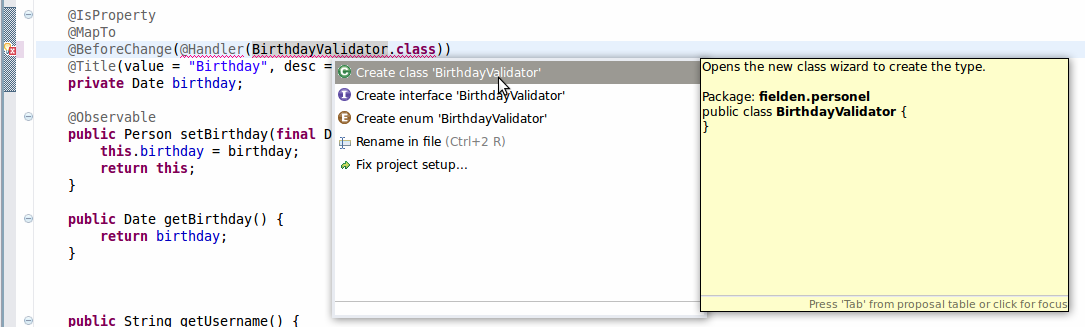
\includegraphics[width=\textwidth]{parts/00-part/chapters/02-making-changes/images/04-create-validator.png}
  \end{image}

  The generated class is an empty class, which does not explicitly extend any other class or implement any contracts\footnote{The term \emph{contract} is used in this book instead of the word \emph{interface} in order not to mix things up when taking about user interfaces and the interface, which is a contract that some class implements.}.
  In order for this class to become a proper \emph{before change event handler}, it needs to implement contract \emph{IBeforeChangeEventHandler}, which requires one type parameter that should match the type of the property.
  In this case, it would be \texttt{Date} to match the type of property \emph{birthday}.
  The contract demands implementation of only one method \emph{handle} that would provide the necessary validation logic.
  
  The \emph{test-first} approach works really well when implementing business logic, which ensures both the correctness of the business logic and the quickest possible implementation time by navigating the development effort along the requirements captured by tests.
  Thus, let's first provide stub implementation for the handler class as illustrated in Listing~\ref{lst:Person-birthday-validation-stub}, and then implement the test that would define that should happen during birthday validation.  
  The stub returns a successful validation result, which is equivalent to not having any validation at all.
  
 \begin{code}{Birthday validation logic stub.}{\label{lst:Person-birthday-validation-stub}}{codebgcolor}
    \begin{lstlisting}
public class BirthdayValidator implements IBeforeChangeEventHandler<Date> {

    @Override
    public Result handle(final MetaProperty property, 
			 final Date newValue, final Date oldValue, 
			 final Set<Annotation> mutatorAnnotations) {
	return Result.successful(newValue);
    }
}
    \end{lstlisting}
  \end{code}
  
  The generated application conveniently provides an example of a domain-driven unit test case for entity Person.
  Open test case \emph{PersonnelTest} by using the \texttt{Open Type} dialog as before in the editor, and without explaining too much of the existing code\footnote{A separate chapter is dedicated to unit testing further in the book.} add the four tests from Listings~\ref{lst:Person-birthday-validation-test-1}-\ref{lst:Person-birthday-validation-test-4} to this test case.

  \begin{notebox}{A rule of thumb.}{\label{mb:rule-of-thumb}}
    Creation of unit tests should follow a rule of thumb where by \emph{each unit test should ensure one particular fact}.
    This keeps tests short in code and clear in meaning.
    The recommended approach is to use test method name to specify what fact it ensures.
    The provided examples follow this rule.
  \end{notebox}  

 \begin{code}{Personnel younger 23 should produce warning.}{\label{lst:Person-birthday-validation-test-1}}{codebgcolor}
    \begin{lstlisting}
@Test
public void birthday_indicating_a_young_person_should_produce_warning() {	
  final Person person = ao(Person.class).
			findByKey("USER2").
			setBirthday(new DateTime().minusYears(20).toDate());	

  assertTrue("Should be valid", 
             person.getProperty("birthday").isValid());
  assertNotNull("Should have warning", 
                person.getProperty("birthday").getFirstWarning());
}
    \end{lstlisting}
  \end{code}

\begin{code}{Personnel younger 23 should be persisted.}{\label{lst:Person-birthday-validation-test-2}}{codebgcolor}
    \begin{lstlisting}
@Test
public void birthday_indicating_a_young_person_should_be_saved() {	
  final Date birthday = new DateTime().minusYears(20).toDate();
  final Person person = ao(Person.class).
			findByKey("USER2").
			setBirthday(birthday);

  ao(Person.class).save(person);

  assertEquals("Incorrectly saved birthday.", 
	  birthday,
          ao(Person.class).findByKey("USER2").getBirthday());
}
    \end{lstlisting}
  \end{code}

  All tests rely on the fact that test data contains a person with business key equals to \texttt{USER2} and property \emph{birthday} that has no value (i.e. it is null).
  Test in Listing~\ref{lst:Person-birthday-validation-test-1} ensures rule \emph{2.a} that if the birth date suggests a person younger than 23 years of age then a warning should be raised, but the value should be recognised as valid.
  Test in Listing~\ref{lst:Person-birthday-validation-test-2} ensures that these ``early'' birthday value are saved correctly.
  Strictly speaking this test is not necessary and is provided only for the purpose of example, as it tests an already established at the platform level fact -- correct property values can be persisted when requested.

  The third test (Listing~\ref{lst:Person-birthday-validation-test-3}) ensures rule \emph{2.b} that no future birth dates are acceptable.
  The last test (Listing~\ref{lst:Person-birthday-validation-test-4}) ensures that invalid birthday value is not saved
  \footnote{Similar to test in Listing~\ref{lst:Person-birthday-validation-test-2}, it is provided more as an example -- the platform does not permit saving of invalid values, and there is no particular reason to test this invariant behaviour at the application level}.

\begin{code}{Unborn personnel should lead to a validation error.}{\label{lst:Person-birthday-validation-test-3}}{codebgcolor}
    \begin{lstlisting}
@Test
public void future_birthday_date_should_produce_validation_error() {	
  final Person person = ao(Person.class).
			findByKey("USER2").
			setBirthday(new DateTime().plusYears(1).toDate());	

  assertFalse("Should be invalid", 
              person.getProperty("birthday").isValid());
}
    \end{lstlisting}
  \end{code}

\begin{code}{Unborn personnel should not be persisted.}{\label{lst:Person-birthday-validation-test-4}}{codebgcolor}
    \begin{lstlisting}
@Test(expected = Result.class)
public void future_birthday_date_should_be_null() {
  final Person person = ao(Person.class).
                        findByKey("USER2").
                        setBirthday(new DateTime().plusYears(1).toDate());
  save(person);
}
    \end{lstlisting}
  \end{code}

  Running these tests by pressing \texttt{Ctrl+F11} combination while in the editor window of the test case, should result in failure of three out of four of the provided tests\footnote{The generated test \texttt{should\_be\_able\_to\_find\_person\_USER2} should also succeed.}.
  Test \texttt{birthday\_indicating\_a\_young\_person\_should\_be\_saved} succeeds because any value without validation is persisted when requested.
  For the same reason, test \texttt{future\_birthday\_date\_should\_not\_be\_saved} fails.

  The provided unit tests establish a set of constraints that guide the coding effort -- once all the tests pass the validation rule implementation can be declared completed.
  Listing~\ref{lst:Person-birthday-validation} provides a complete validation logic that satisfies all business requirements.
  Before moving further in the text please try to implement the validation rules personally without using code from the listing to make the tests pass.


 \begin{code}{Birthday validation logic}{\label{lst:Person-birthday-validation}}{codebgcolor}
    \begin{lstlisting}
public class BirthdayValidator implements IBeforeChangeEventHandler<Date> {

    @Override
    public Result handle(final MetaProperty property, 
			 final Date newValue, final Date oldValue, 
			 final Set<Annotation> mutatorAnnotations) {
	if (newValue != null) {
	    // let's use Joda Time for intermediate calculations
	    final DateTime date = new DateTime(newValue);
	    // reject future dates 
	    if (date.isAfterNow()) {
		return new Result(newValue, 
	                          new IllegalArgumentException("Cannot be in future."));
	    }
	    // warn if younger than 23 years of age 
	    if (date.isAfter(new DateTime().minusYears(23))) {
		return new Warning("The person is potentially too young.");
	    }
	}	
	
	return Result.successful(newValue);
    }
}
    \end{lstlisting}
  \end{code}

\subsection{Modifying User Interface}
  In order for application users to be able to enter and modify values of the \emph{birthday} property added to the \emph{Person} entity, the application user interface (UI) needs to be updated.
  A complete discussion of the UI development support as provided by the platform is presented in chapter~\ref{?}.
  In this section we only cover the most essential concepts required to gain a general understanding in order to add \texttt{birthday} property to the application UI.

  The platform's UI programming model is based on Model-View-Presenter (MVP) pattern~\cite{BoGl2000}, which in turn is an improvement to the well known Model-View-Controller (MVC) pattern.  
  In order to align the MVP nomenclature with the nomenclature of the platform, it was renamed into Domain-Model-View (DMV):
  \begin{description}
    \item[\textbf{The Domain.}] Represents a pure business domain model with entities and controllers that bares no UI logic\footnote{This separation of concerns is ensured at the module level, where business controller have no visibility of UI code.}.
    \item [\textbf{The Model.}] Governs how the domain can be manipulated and changed from UI. 
	This is where the heart of the application UI logic resides. The view and model can closely collaborate in their roles of supplying the user interface for a particular domain.
    \item[\textbf{The View.}] Has the responsibility to display the content of a domain. 
	It is represented in TG by property editors and specialised containers (panel or frame) for holding UI controls.    
  \end{description}

  The platform provides a wide range of models and views that can be used as the basis for building consistent user interface.
  Let's quickly have a look at the basic modus operandi for developing UI for entering and editing \emph{Person} entities.
  \begin{description}
    \item[\textbf{Domain identification.}] Identify the part of the domain to be represented by UI. 
	For example, if we need to build a master UI for entering/modifying of \emph{Person} then entity type \emph{Person} together with a corresponding controller \emph{IPerson}, which is specified using annotation \texttt{DefaultController}, represent the required domain part.
    \item [\textbf{UI Model construction.}] Construct a UI model, which should be a new class extending one of the provided UI models. 
	In case of a master it would be either \emph{UmMasterWithCrud} or one of its descendants. 
	For example, a master model for \emph{Person} is implemented by class \emph{PersonMasterModel}, which extends \emph{UmMasterWithCrudAndUpdater\textless Person, IPerson\textgreater}. 
	Type parameterisation plays a important role to support type aware UI models that ensures type safety.
	UI models can be composed together in order to form more complex models for supporting composition of UI views.
    \item[\textbf{UI View construction.}] Construct a UI view for the provided UI model. 
	Each UI view is a container. 
	Views can be composed to provide sophisticated user interfaces that could bringing together loosely coupled business domain concepts into one UI view.
	At the very least UI views should extend either \emph{BasePanel} (a compoundable container, is embedded into other views) or \emph{BaseFrame} (a final container, may hold other views) classes. 
	In most cases more specialised classes that are provided by the platform should be used.
	For example, a view for the \emph{Person} master is represented by \emph{PersonMasterView} derived from \emph{MasterPanel}, which has a tree menu and embeds view \emph{PersonMainView} that can be accessed via one of menu's items.
	The \emph{PersonMainView} view is derived from \emph{BaseNotifPanel\textless PersonMasterModel\textgreater} parameterised with the aforementioned UI model.
  \end{description}
  
  Class \emph{PersonMainView} represent the UI view, which needs to be modified in order to provide application users with ability to change person's birthday.
  Its method \emph{buildUi} contains the layout logic of UI elements displayed by the view.
  Listing~\ref{lst:person-main-view-before-change} shows the beginning of this method.
  Line~3 declares a \emph{JPanel} instance, created with a \emph{MigLayout}\footnote{Any Swing layout manager can be used instead, but we strongly recommend to use MigLayout as a one-stop solution for all layouting needs. 
	    The platform layouting support inherently based on MigLayout. 
	    In a chapter on UI we'll provide more details about the provided support and flexibility of MigLayout.} 
  layout manager.
  The specified layout settings ensure the following:
  \begin{itemize}
    \item The panel has no insets (i.e. the gap between the edges of the panel and the embedded elements is zero).
    \item There are two columns -- one with preferred width of 50 units, another -- should be filled with embedded component (the \texttt{fill} option) and should resize that component if the width of the column changes (the \texttt{grow} option).
    \item There can be any number of rows with their content centred.
  \end{itemize}

 \begin{code}{PersonMainView code before modification.}{\label{lst:person-main-view-before-change}}{codebgcolor}
    \begin{lstlisting}
@Override
public void buildUi() {
    final JPanel componentsPanel = new JPanel(new MigLayout("insets 0", 
						  "[:50:][grow, fill]", 
						  "[c]"));
    final Map<String, IPropertyEditor> editors = getModel().getEditors();
    ///////////////////////////////////////////////////////    
    addAndWrap(componentsPanel, editors, "key"); // row 1
    addAndWrap(componentsPanel, editors, "desc"); // row 2
    ...
}
    \end{lstlisting}
  \end{code}

  The platform provides a convenient abstraction for UI components that are used to change property values of domain entities.
  It is called \emph{Property Editor}.
  Thus, there is no need to work directly with low level UI components such as text fields, labels and date pickers, which would require tremendous effort to build a user interface (consider the matter of binding components to entity properties, handle validation and error etc.).
  Instead, the platform automatically determines what UI components are most appropriate for any given property based on its type and constructs an instance of a higher-order UI component -- a property editor.
  Property editors are bound to corresponding properties, so if user changes value from UI it is propagated to the property and vice versa -- if a property is changed programmatically its value is automatically refreshed in UI.
  They take full advantage over the associated with properties meta-data such as validation logic, title, description etc. 
  This approach completely removes the dichotomy of the UI and business logic -- in all cases the domain determines the behaviour.
  
  Line~6 declares a variable, which points to a map of all \emph{property editors} obtained from a corresponding UI model.
  Due to the fact that the UI model is associated with domain entity \emph{Person}, this map contains editors for all of its properties.

  Lines~8 and 9 invoke an inherited from the base view class method \emph{addAndWrap} to add editors for properties \emph{key} and \emph{desc} to two sequential rows on the view.
  At the surface a property editor is very simple.
  It has two principle parts -- a label component and an editor component.
  Method \emph{addAndWrap} reuses this to place property label into the first column of the layout and the editor -- into the second column.
  The result is depicted in Fig.~\ref{img:ch00:03:person-main-before-change}.

  \begin{image}{PersonMainView L\&F before modification.}{\label{img:ch00:03:person-main-before-change}}
    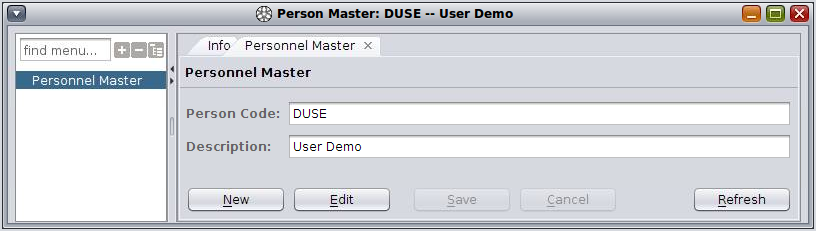
\includegraphics[width=0.9\textwidth]{parts/00-part/chapters/02-making-changes/images/05-person-main-before-change.png}
  \end{image}

  As can be suspected based on the above information, enabling application users to enter and change person birthday is a matter of a very simple change -- adding birthday property editor to the view.
  Listing~\ref{lst:person-main-view-after-change} shows a modified code, where method \emph{addAndWrap} is used on line 10 to add birthday property editor to the view below the existing editors.

 \begin{code}{PersonMainView code after modification.}{\label{lst:person-main-view-after-change}}{codebgcolor}
    \begin{lstlisting}
@Override
public void buildUi() {
    final JPanel componentsPanel = new JPanel(new MigLayout("insets 0", 
						  "[:50:][grow, fill]", 
						  "[c]"));
    final Map<String, IPropertyEditor> editors = getModel().getEditors();
    ///////////////////////////////////////////////////////    
    addAndWrap(componentsPanel, editors, "key"); // row 1
    addAndWrap(componentsPanel, editors, "desc"); // row 2
    addAndWrap(componentsPanel, editors, "birthday"); // row 3
    ...
}
    \end{lstlisting}
  \end{code}  

  The result is depicted in Fig.~\ref{img:ch00:03:person-main-before-change}.

  \begin{image}{PersonMainView L\&F after modification.}{\label{img:ch00:03:person-main-after-change}}
    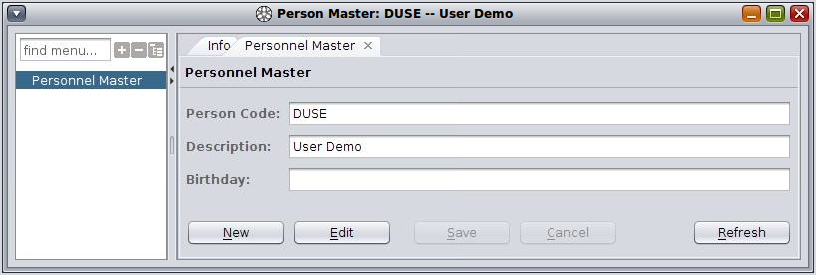
\includegraphics[width=0.9\textwidth]{parts/00-part/chapters/02-making-changes/images/06-person-main-after-change.png}
  \end{image}

  In order to fully appreciate the power of such a trivial change, let's run the application.
  But first, we need to update the development database to reflect the fact of adding a new persistent property \emph{birthday} to entity \emph{Person}.
  This is covered in the next section.
  

\subsection{Running the Modified Application}

  When a business domain model changes in ways that require changes to the underlying database\footnote{This is mostly related to creation of new persistent domain entities or addition/removal/modification of properties for existing persistent domain entities.}.
  The proper way of initiating and tracking such changes during production application development is covered in a separate chapter of this book.
  For pure development convenience, the generated application provides a utility, which should be used for autoupdate of the development database.
  Similarly as for data-aware unit tests, it is always a good thing to be able to set the development database into a known state.
  The provided development utility should be used for exactly this purpose.
  This way, regardless of how you modify the data in the development database when running an application, it is always possible to reset it to the predefined state.

  Open the utility main class \emph{PopulateDb} via an \texttt{Open Type} dialog (\texttt{Ctrl+Shit+T}) in the code editor.
  This class extends the provided by platform class \emph{DomainDrivenDataPopulation} by overriding its method \emph{populateDomain} in order to define application specific data state.
  Running this class changes the development database based on the current domain definition and populates the state as specified in method \emph{populateDomain}.

  At this stage we do not need to change the initial data.
  Thus, simple execute the class by pressing \texttt{Ctrl+F11} key combination to recreate the database in order to provide the newly added property \emph{birthday} of entity \emph{Person} with a column.
  Before running the utility, please make sure that the application server is shutdown as it would locks the H2 development database, which runs in file mode.
  Once the utility finishes, we can start the server followed by the client in order to observe changes made in the previous section.

  When the client is up and running (a login prompt should be presented due to the database reset), navigate to the \emph{Personnel} main menu item in the \emph{Table Codes} group\footnote{Another way is to simply start typing item's title in the search bar above the main menu tree.}.
  Open it -- this is an entity centre for entity \emph{Person} -- and configure to add property \emph{birthday} both as the selection criteria and result as depicted in Fig.~\ref{img:ch00:03:person-centre-configuration}.
  The configuration result is depicted in Fig.~\ref{img:ch00:03:person-centre}.

  \begin{image}{Person centre configuration.}{\label{img:ch00:03:person-centre-configuration}}
    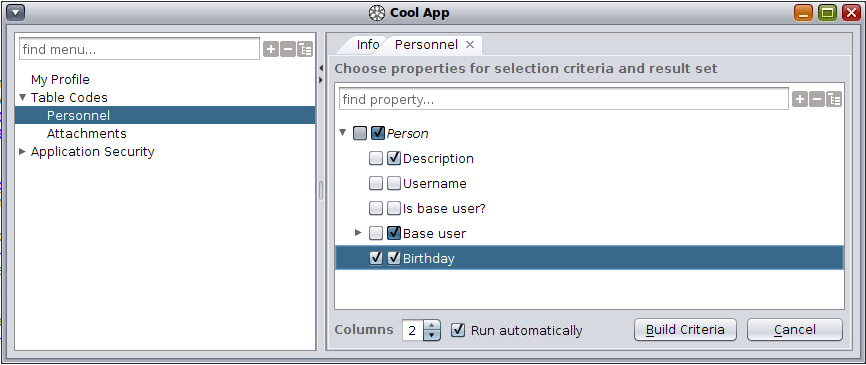
\includegraphics[width=0.9\textwidth]{parts/00-part/chapters/02-making-changes/images/07-person-centre-configuration.png}
  \end{image}

  \begin{image}{Person centre with birthday.}{\label{img:ch00:03:person-centre}}
    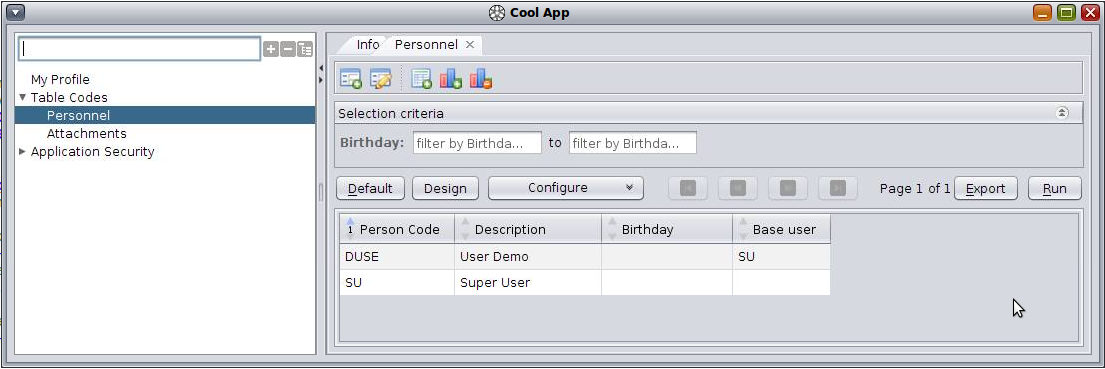
\includegraphics[width=\textwidth]{parts/00-part/chapters/02-making-changes/images/08-person-centre.png}
  \end{image}

  This shows that declaring property \emph{birthday} as part of \emph{Person} automatically propagated it to the generic UI facilities such as Entity Centres without any additional work.
  
  Double clicking \emph{Person Code} with value \texttt{DUSE} in the resultant grid (Entity Grid Inspector, EGI) of the Person Centre should invoke a master view for entity \emph{Person}, which we modified in the previous section.
  Click the \emph{Edit} button on the invoked master, focus the \emph{birthday} editor.
  This activates the date/picker button at the right end of the editor, which can be used to visually enter the date value.
  Figure~\ref{img:ch00:03:person-master-editing} depicts date selection for property \emph{birthday}.

  \begin{image}{Person birthday entry.}{\label{img:ch00:03:person-master-editing}}
    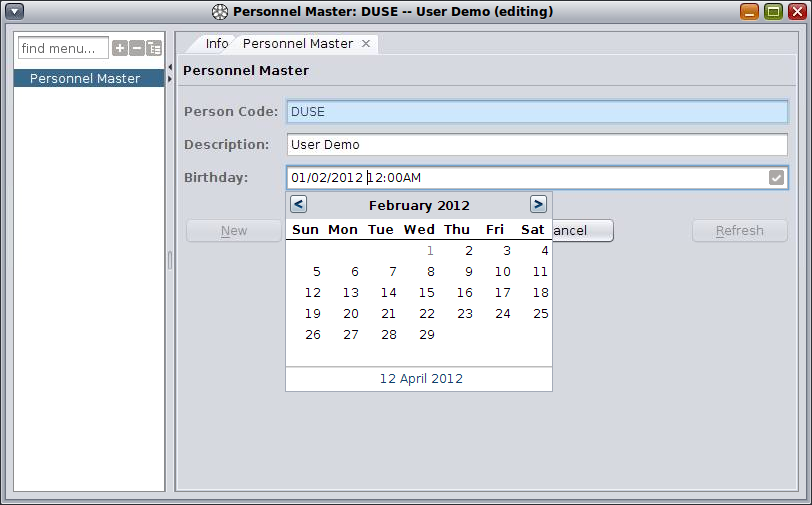
\includegraphics[width=0.9\textwidth]{parts/00-part/chapters/02-making-changes/images/09-person-master-editing.png}
  \end{image}
  
  Please recall the validation rules for the birthday in section \ref{ch00:03:the-scenario}.
  Try setting future value (invalid) and a value less than 23 into the past (warning), and observe how UI reacts\footnote{Please note that for the entered value to be set, the editor needs to loose focus.}.
  Point the mouse cursor to the highlighted editor (red -- indicates error, yellow -- warning) to see the reason for an error and warning.
  Figures~\ref{img:ch00:03:person-master-warning} and \ref{img:ch00:03:person-master-error} depict the cases with warning and error respectively.
  
  Thus, with a one line modification to UI, the applications gains all necessary functionality for entering/changing the \emph{birthday} value and follows all the domain rules defined for this property automatically.
  
  \begin{image}{Person birthday warning.}{\label{img:ch00:03:person-master-warning}}
    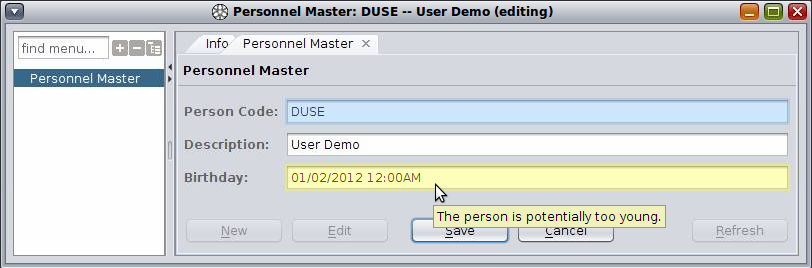
\includegraphics[width=0.9\textwidth]{parts/00-part/chapters/02-making-changes/images/10-person-master-warning.png}
  \end{image}

  \begin{image}{Person birthday entry.}{\label{img:ch00:03:person-master-error}}
    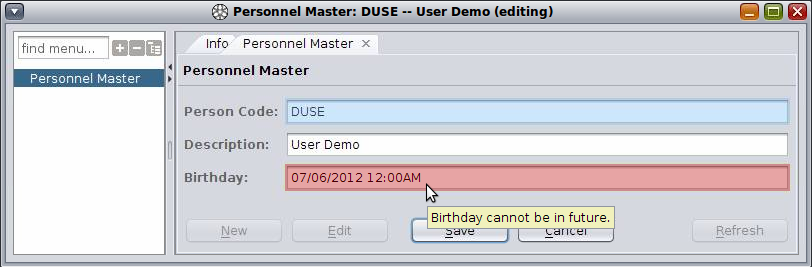
\includegraphics[width=0.9\textwidth]{parts/00-part/chapters/02-making-changes/images/11-person-master-error.png}
  \end{image}
  
\subsection{Securing the Access}

  At the end of this chapter, let's quickly show how easy it is to secure the capability to modify the \emph{Person} property \emph{birthday}.

  \subsubsection*{Security token creation}
  The first step for this is to create a \emph{security token}\emph{A separate chapter on security provide full discussion, which cannot be included into the quick start.}, which should implement contract \emph{ISecurityToken}.
  All security tokens should be a part of \texttt{coolapp-pojo-bl} module.
  It is advised to keep all security tokens in subpackages of the same dedicated parent package.

  The generated application already contains a number of security tokens, some of which guard \emph{Person} related functionality.
  All security token are located in subpackages on package \texttt{fielden.security.tokens}.
  Personnel related tokens are located in package \texttt{fielden.security.tokens.personnel}.
  
  Security tokens can form a hierarchy, which is recognised at runtime by the security functionality when presenting tokens to the user for management.
  For example, security token \emph{PersonnelReviewToken}, which implements \emph{ISecurityToken}, servers as the root type for all tokens related to personnel review capabilities.
  Annotation \emph{KeyTitle} should be used to specify how any particular security token should appear to application users.
  This is the same annotation used for providing title and description for domain entities.

  Let's create a new security token with a root specified as an existing \emph{PersonnelReviewToken} by creating a new class \emph{PersonBirthdayToken} in package \texttt{fielden.security.tokens.personnel}, which extends class \emph{PersonnelReviewToken}.
  This new class should be annotated with \emph{KeyTitle} provided with appropriate \emph{value} and \emph{desc}.
  Listing~\ref{lst:person-birthday-token} shows the token's implementation.

 \begin{code}{PersonMainView code after modification.}{\label{lst:person-birthday-token}}{codebgcolor}
    \begin{lstlisting}
package fielden.security.tokens.personnel;
...
@KeyTitle(value = "Person birthday", 
	  desc = "Controls permission to change person's property birthday.")
public class PersonBirthdayToken extends PersonnelReviewToken {
}
    \end{lstlisting}
  \end{code}  
  
  \subsubsection*{Securing property \emph{birthday}}
  The next step is to associated the created security token with a setter of property \emph{birthday}.
  Navigate to class \emph{Person} and change setter \emph{setBirthday} as illustrated in Listing~\ref{lst:Person-birthday-auth} -- line 2 specifies authorisation annotation with an argument set to just created security token type \emph{PersonBirthdayToken}.

  \begin{code}{Property \emph{birthday} authorisation.}{\label{lst:Person-birthday-auth}}{codebgcolor}
    \begin{lstlisting}
    @Observable
    @Authorise(PersonBirthdayToken.class)
    public Person setBirthday(final Date birthday) {
      this.birthday = birthday;
      return this;
    }
    \end{lstlisting}
  \end{code}

  \subsubsection*{Look ma, I cannot change my \emph{birthday}}
  In order to observe the effect of this change restart the client and server and try changing property \emph{birthday} on the \emph{Person} master.
  This should not be possible as the newly created security token is not marked as authorised for the user role of the currently logged in user \texttt{SU}.
  Fig.~\ref{img:ch00:03:person-master-birthday-permission} depicts a corresponding error.
  
  \begin{image}{Person birthday permission error.}{\label{img:ch00:03:person-master-birthday-permission}}
    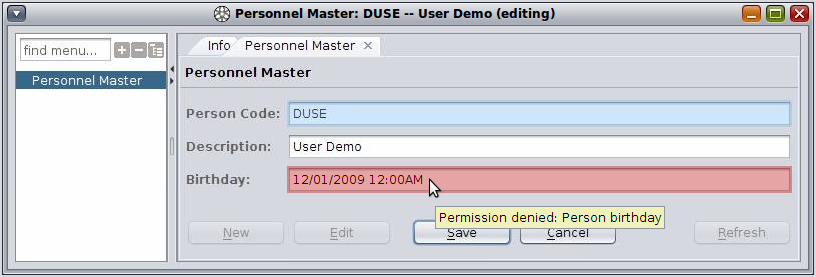
\includegraphics[width=0.9\textwidth]{parts/00-part/chapters/02-making-changes/images/12-person-master-birthday-permission.png}
  \end{image}

  Due to the fact that \texttt{SU} user has permission to change change security token permissions, please grand \emph{Person birthday} token to the role \emph{ADMINISTRATOR}.
  This can be done by using \emph{Token/Role Management} facility, available as part of the application.
  Figure~\ref{img:ch00:03:person-birthday-permission} depicts the state of token/role associations before granting access to \emph{Person birthday}.

  \begin{image}{Person birthday token association with use role.}{\label{img:ch00:03:person-birthday-permission}}
    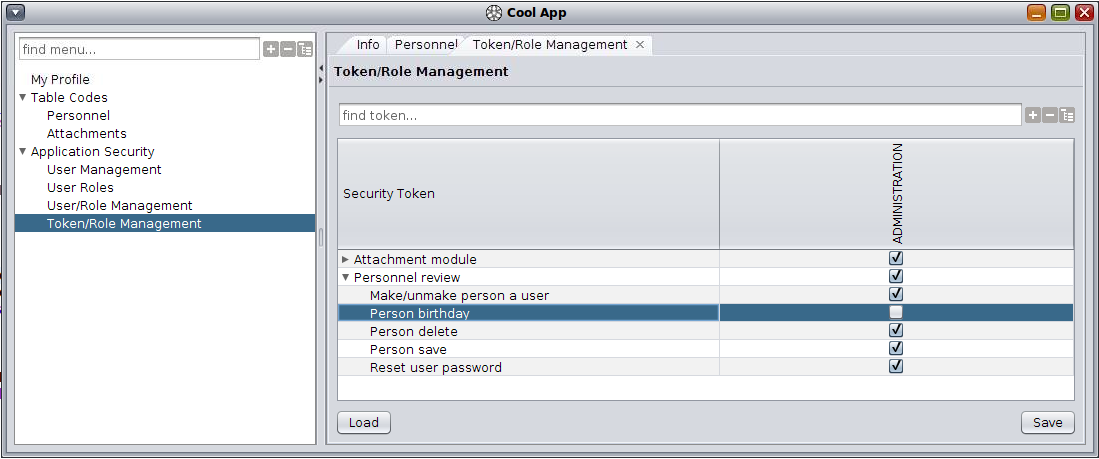
\includegraphics[width=0.9\textwidth]{parts/00-part/chapters/02-making-changes/images/13-person-birthday-permission.png}
  \end{image}

  Once \emph{Person birthday} has been associated with role \emph{ADMINISTRATOR} (click a corresponding checkbox and press the \emph{Save} button), there should be no problems changing the \emph{birthday} property (no application restart is necessary).